
\subsection{Use Case Diagram}
\begin{figure}[h]
    \centering
    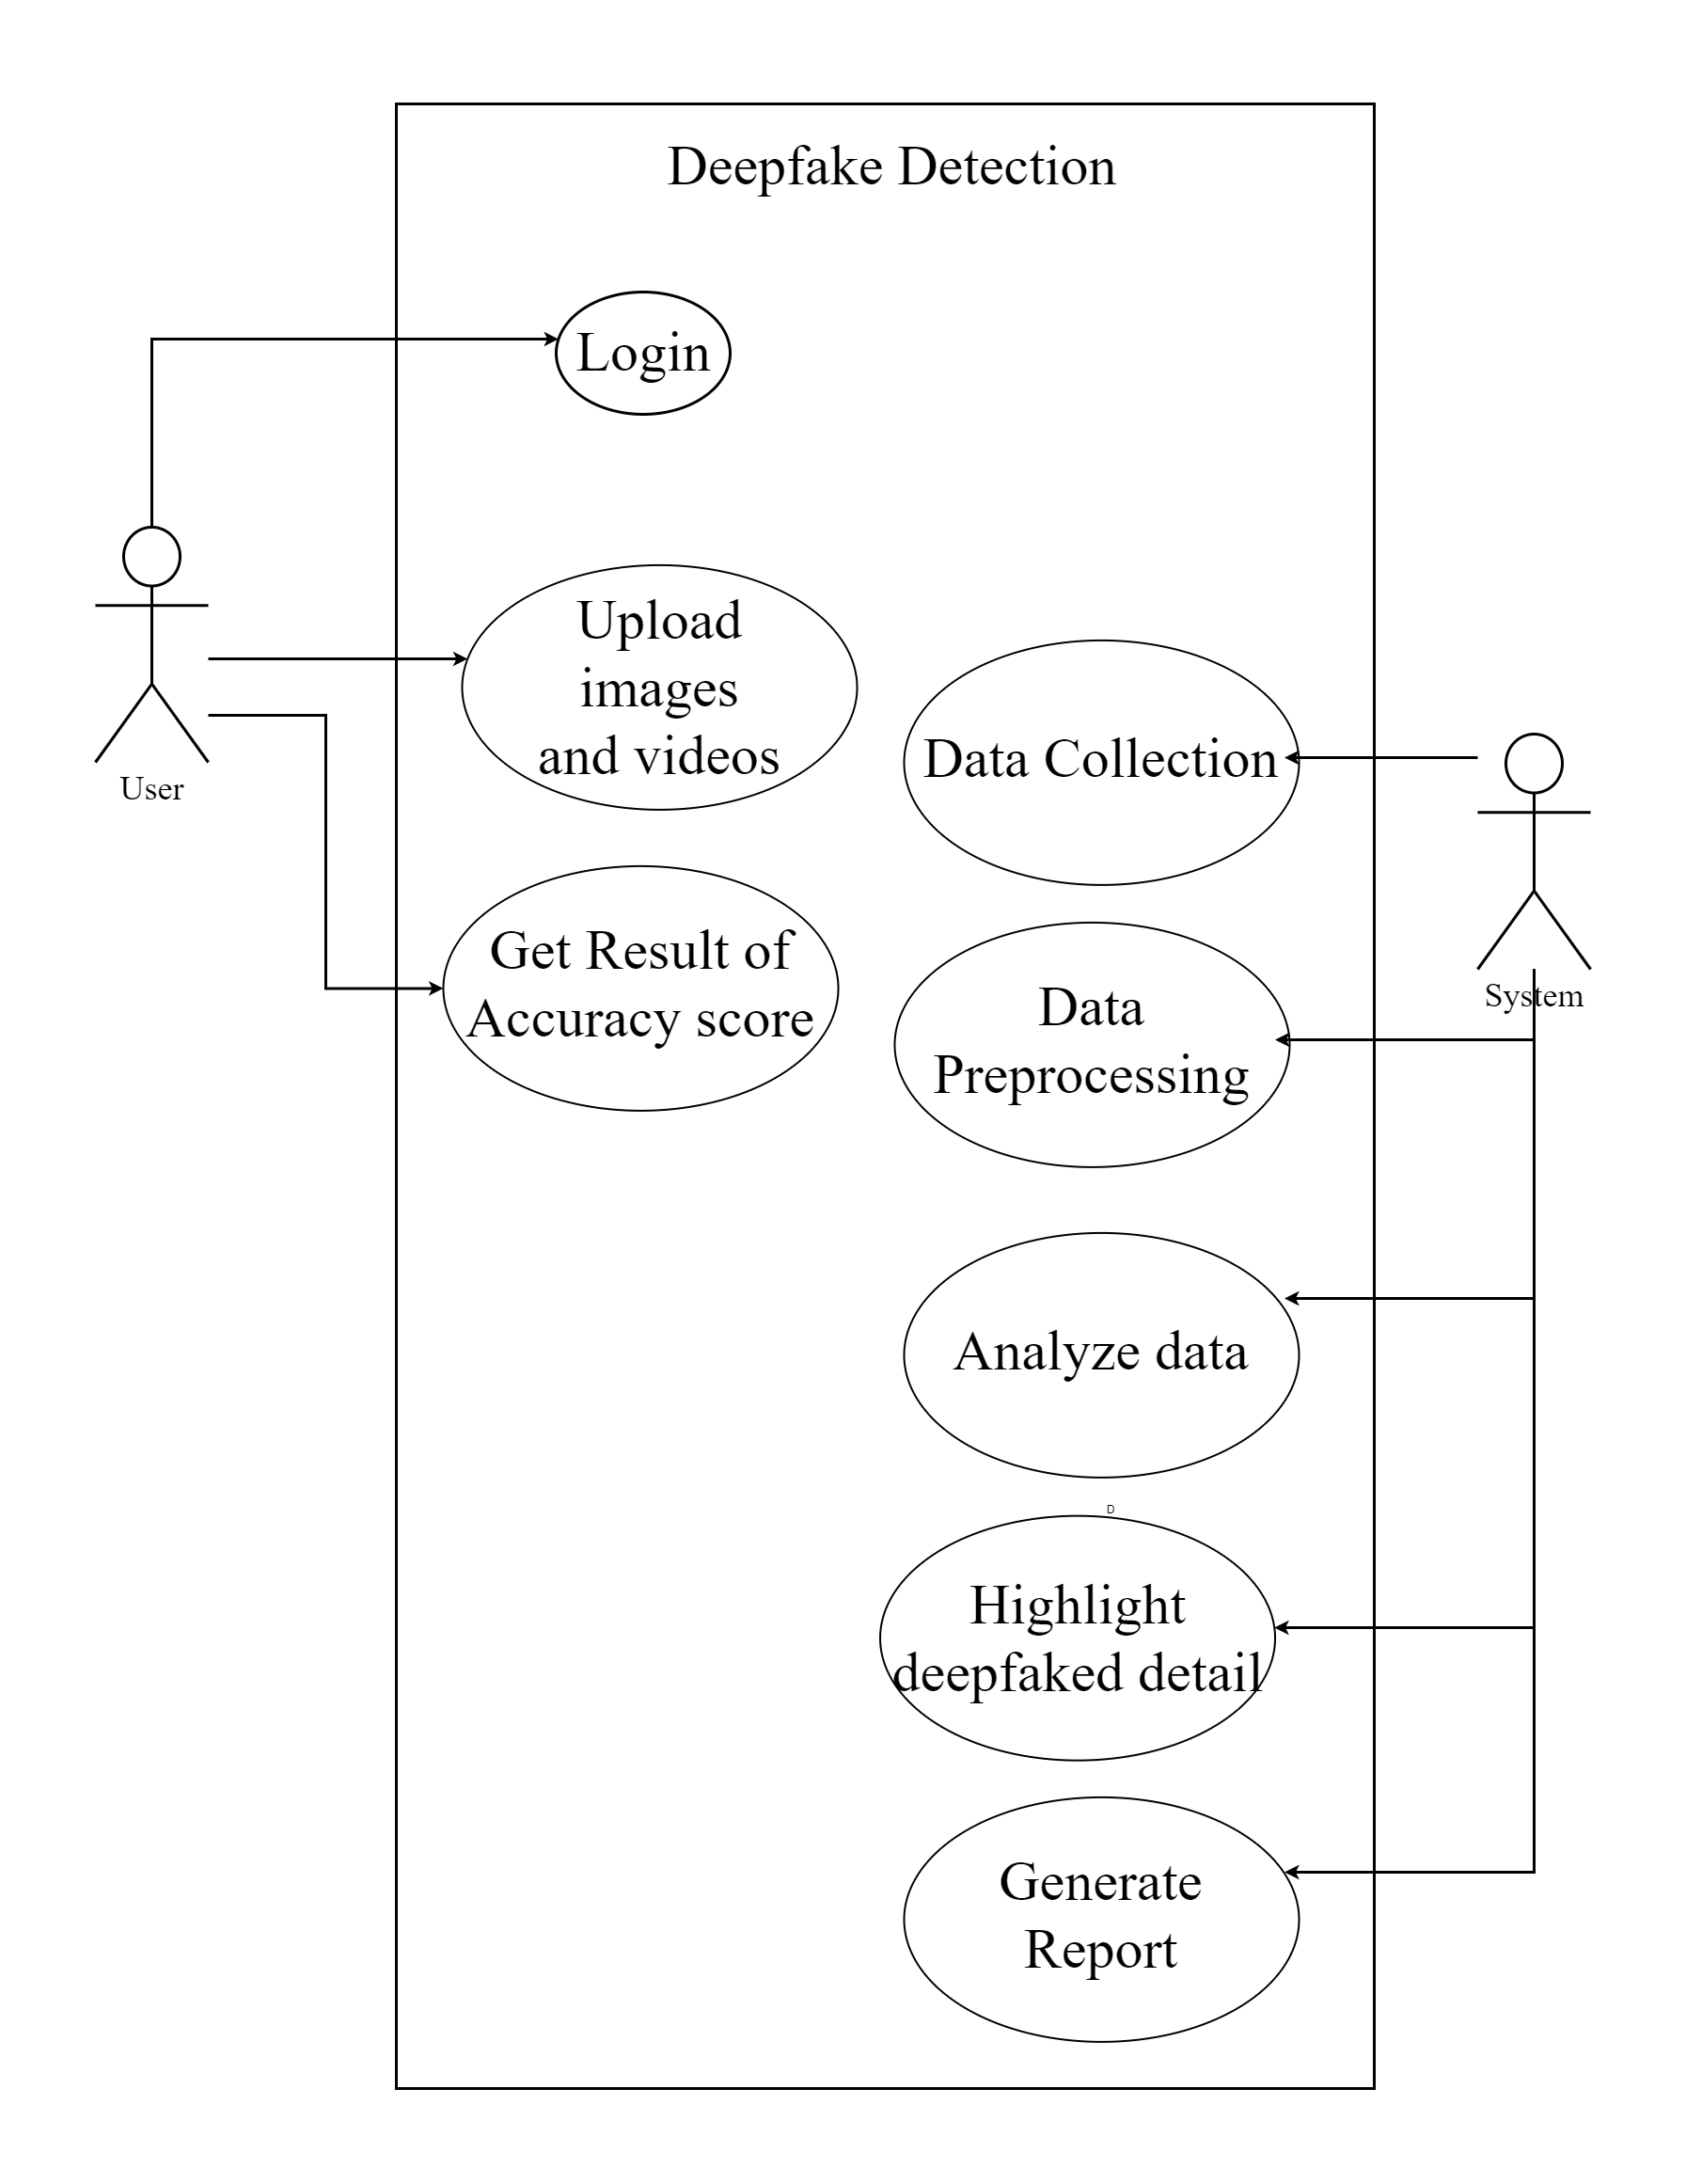
\includegraphics[width= 5in ]{img/usecasediagram.drawio.png}
    \caption{\textit{Use Case Diagram}}
\end{figure}
\justify
The use case diagram for our system illustrates various interactions and roles of the system's users. The primary actors involved are the "User" and the "System." The User interacts with the system by initiating the deepfake detection process, either by uploading a video or an image. The User can also access the system to view the detection results. On the other hand, the System is responsible for managing the system, including user authentication, system configuration, and monitoring the overall functionality. The use case diagram shows the main use cases, such as "Upload Media," "Detect Deepfake," and "View Results," which represent the key functionalities of the system.